\chapter{Implementierung}
In Abstimmung mit CGM wurde das Konzept aus Kapitel 3 für die Umsetzung gemäß Zielsetzung herangezogen. Dabei wurden die Funktionen der EWS-API verwendet und in den Methoden der nachfolgenden Module aufgerufen: 
\section{Microsoft Outlook}
Die nachfolgenden aufgelisteten Packages beziehen sich auf die Klassen: 
	 \textit{Packagename + Service },
	 \textit{I + Packagename + Service} und
	\textit{Packagename + Dto} (siehe Klassendiagramm Abb. 4.1)

Die jeweilige Klasse des Packages implementiert eine vordefinierte Schnittstelle (Interface), welche einen vordefinierten Benennungsschema folgt. Die Funktionalitäten sind unabhängig vom MRP-System, können aber von diesem verwendet werden. Die für die Arbeit entwickelten Datentypen sind im Package \textit{Model} definiert. Diese Klassen können gleichnamige Klassen im MRP haben, haben aber keine Beziehung zu diesen Klassen. \\


	\begin{figure}[H]
	\centering
\noindent\makebox[\textwidth]{%
		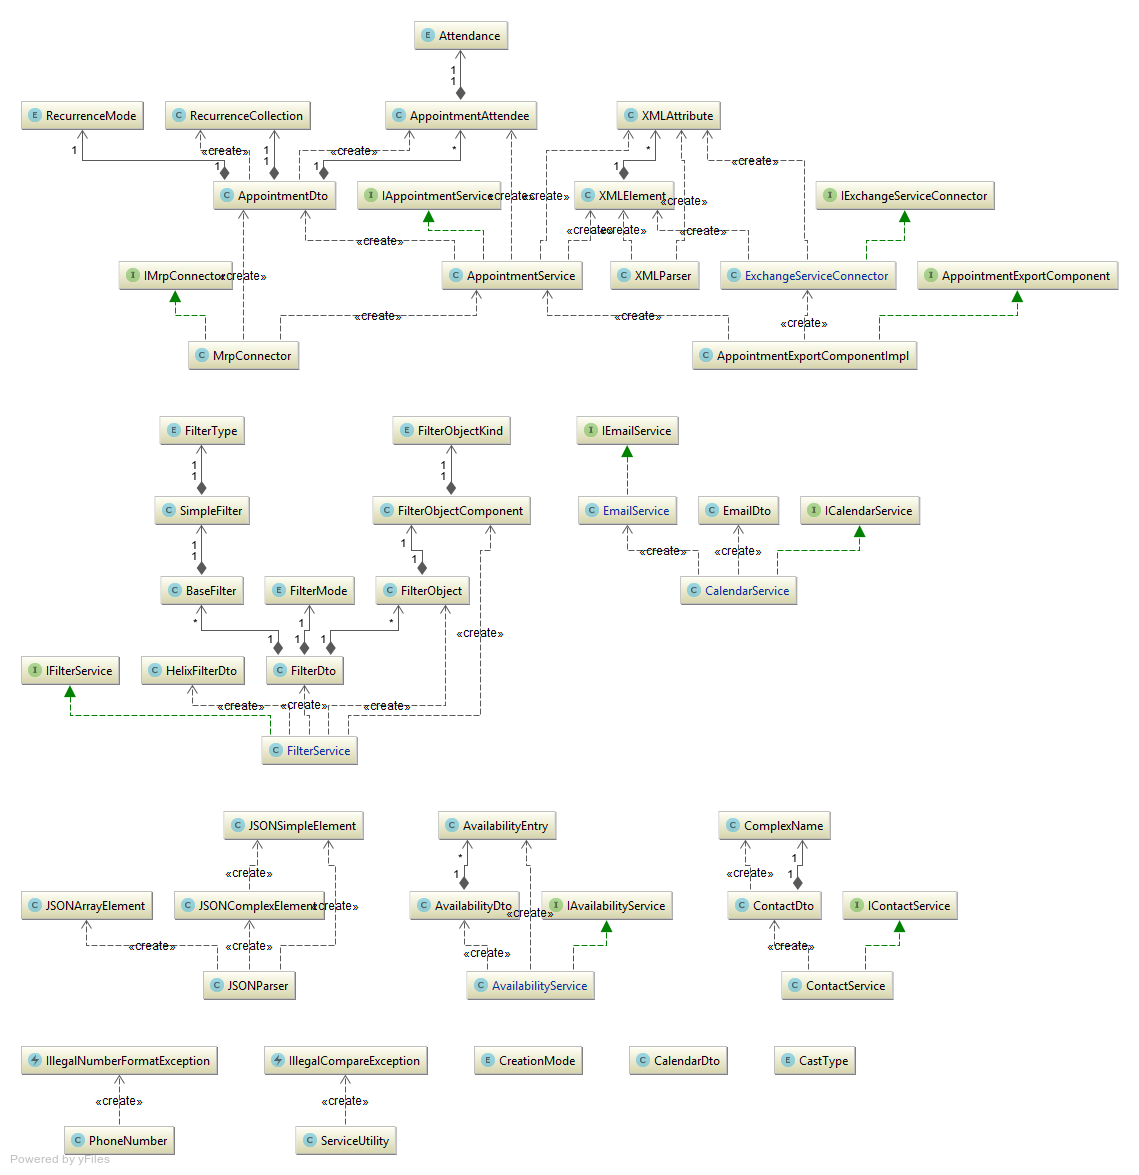
\includegraphics[width=1.2\textwidth]{diagram.png}}
\caption{Klassendiagramm}
\end{figure}


\subsection{Exchangeservice}
Der Exchangeservice dient als zentrale Verbindung zum Microsoft Outlook. Die Features bzw. Methoden, welche mit dem Exchange-Server kommunizieren, verwenden ExchangeService als Parameter. Die Klasse wird \textit{ExchangeServiceConnector} genannt und ist zuständig für die Verbindung zum Server sowie für die Anfragen der Features. Dieser Service bezieht sich ausschließlich auf das eigene Outlookkonto bzw. auf das Konto, welches mit Passwort und Benutzername angegeben wird. Weiters besteht die Möglichkeit die Exchangeserverversion festzulegen. Diese Klasse implementiert das zugehörige Interface \textit{IExchangeServiceConnector}.\\ Die Serververbindung wird mit Hilfe der Methode \textit{createServerConnection} initialisiert, wobei der Benutzername und das Passwort als Parameter übergeben werden. Die gleichnamige Methode verwendet zusätzlich den Parameter Server-URL. Die Methode \textit{createServerConnection} baut mit Hilfe der Daten eines XML-Dokuments eine Serververbindung auf. Die genanten Methoden retournieren eine Instanz des Exchangeservice. Dieser Service existiert nur einmal zur Laufzeit. Damit wird garantiert, dass immer der gleiche Server angesteuert wird. Mit der Methode \textit{saveSettingsToXML} können die Servereinstellungen in einem XML-Dokument gespeichert werden. 
\subsection{Model}
Die verwendeten Objekte bzw. Datentypen in den einzelnen Features bzw. Packages werden im Model repräsentiert. Die einzelnen Klassen repräsentieren die jeweiligen Datentypen, welche einer vordefinierten Struktur folgen. Diese folgt der Bean-Definition. Diese bedeutet, dass alle Membervariablen \textit{private} sind und daher wird auf die Variablen mit Getter und Setter zugegriffen. Die einzelnen definierten Datentypen besitzen einen öffentlichen Default-Konstruktor ohne Parameter.
\subsection{Kalender}
Mittels Kalenderservice können Kalender angelegt und abgerufen werden. Der \textit{CalendarService} implementiert das zugehörige Interface \textit{ICalendarService} und verwendet den Datentyp \textit{CalendarDto}.\\ Die Mehode \textit{getCalendars} ruft die verfügbaren Kalender einer Emailadresse ab. Die Emailadresse repräsentiert Personen oder Räume. Zusätzliche Kalender werden durch die Methode \textit{createNewCalendar} angelegt. Auch gibt es die Methode \textit{sendWarningToUser}, mit dieser kann ein Email an den betreffenden Benutzer versendet werden. Die Emailnachricht enthält die betreffende Warnung.
\subsection{Appointments}
Mit Hilfe des Appointmentservices können Microsoft Outlook-konforme Appointments angelegt, verwaltet und abgerufen werden. Weiters ist möglich Appointments in einem XML-Dokument zu speichern. Das XML Dokument beinhaltet die Datenfelder aus dem \textit{Model} in einer validen XML-Struktur. Diese XML-Dokumente können zur Erstellung von Appointments verwendet werden. Es besteht die Möglichkeit Konflikte zu betreffenden Appointments vom Server abzufragen. Der \textit{AppointmentService} implementiert das zugehörige Interface \textit{IAppointmentService} und verwendet den Datentyp \textit{AppointmentDto}. \\ Mit der Methode \textit{createAppointment} kann ein Appointment angelegt werden. Der \textit{ExchangeService} wird als Parameter übergeben. Die Methode \textit{buildAppointment} erstellt den Datentyp \textit{Appointment}. Die Methode \textit{createAppointments} ermöglicht das gleichzeitige Speichern und Anlegen von Appointments. Eine weitere Funktionalität ist durch die Methode \textit{hasConflictedAppoinments} gegeben. Diese Funktion überprüft mit Hilfe des Exchangeservers Konflikte bei betreffenden Appointments. Die Funktionen \textit{appointmentListToXML}, \textit{xmlToDto} und \textit{xmlToAppointmentList} ermöglichen die Verwaltung von outlookkonformen Appointments mithilfe von XML.
\subsection{Availability}
Durch den Availabilityservice können Verfügbarkeiten von Personen und Räumen abgefragt werden. Der \textit{AvailabilityService} implementiert das zugehörige Interface \textit{IAvailabilityService} und verwendet den Datentyp \textit{AvailabilityDto}. \\ Die Hauptfunktion \textit{checkAvailability} ruft mit Hilfe des \textit{ExchangeService} Verfügbarkeiten über die EWS-Schnittstelle ab. Die Methode \textit{checkAvailbilityForPerson} überprüft die Verfügbarkeit von  Personen anhand deren Email-Adressen. Mit Hilfe der Methode \textit{checkAvailbilityForRooms} können im Gegensatz zur obengenannten Methode anstelle von Personen Räume abgefragt werden. Die beiden Funktionen \textit{getRoom} und \textit{getAllRooms} liefern Räume zurück.  Personen und Räume werden durch die jeweiligen Emails repräsentiert.
\subsection{Kontakt}
Der Kontaktservice ermöglicht das Anlegen, Abrufen und Verwalten von Outlookkontakten in den jeweiligen persönlichen Adressbüchern. Der Kontaktservice arbeitet mit dem Benutzer des Exchangeservices. Der \textit{ContactService} implementiert das zugehörige Interface \textit{IContactService} und verwendet den Datentyp \textit{ContactDto}.\\ Die Methode \textit{getContacts} ruft persönliche Kontakte des angemeldeten Benutzers aus dem persönlichen globalen Adressbuch ab. Die Kontakte sind unsortiert und können mittels Filter zusätzlich gefiltert werden. Neue Kontakte werden über die Funktion \textit{buildContact} erstellt. Die Funktion \textit{getContactDtos} liefert mithilfe der Funktion \textit{buildContact} eine Liste vom vordefinierten Datentyp \textit{ContactDto}. 
\subsection{Email}
Der Emailservice ermöglicht das Senden von bestehenden Emails. Diese beinhalten die relevanten Felder der Emails. Weiters können die Emails aus dem jeweiligen Postfach des Benutzers aufgerufen werden. Der \textit{EmailService} implementiert das zugehörige Interface \textit{IEmailService} und verwendet den Datentyp \textit{EmailDto}.\\ Durch die Mehode \textit{sendEmail} können Emails versendet werden. Diese werden in der Mehode \textit{buildEmail} erstellt und enthalten alle relevanten Informationen zu Sender und Empfänger sowie Betreff und Emailtext. Die Methode \textit{getEmails} ruft eine vordefinierte Anzahl Emails aus dem Posteingang ab. 
\subsection{Filter}
Die Filter bestehen aus Filterkomponenten, welche vordefiniert sind. Diese Filterkomponenten folgen dem Prinzip der überpersistenten Speicherung. Dies bedeutet, dass bereits gefilterte Daten trotzdem erhalten bleiben. Grundsätzlich ist jede Filterkomponente aus zwei Teilen aufgebaut: Der erste Teil beinhaltet die Informationen zu den Filtern. Der zweite Teil stellt eine Datensammlung dar. Diese Daten bleiben solange erhalten solange die Filterkomponenten aktiv sind. Die Filterkomponenten werden gleichzeitig bzw. hintereinander angewendet, um die logischen Funktionen AND und OR zu repräsentieren Eine weitere Funktionalität ist der Vergleich von Methoden mit den Variablen.\\ Die Mehode \textit{apply} beschreibt die Hauptfunktionalität des Filters und beinhaltet die Funktionalität, die zur Anwendung eines bestimmten Filters erforderlich ist. Das \textit{FilterDto} beinhaltet sowohl die Filterkomponenten als auch die zu filternden Daten. Mit der Methode \textit{applySimpleFilter} wird ein Filter für eine Sammlung von zu filternden Objekten angewandt. Die Funktion \textit{applyFilter} wird verwendet, wenn die zu filternden Objekte den Typ \textit{AppointmentComponent} darstellen. Die zwei Funktionen \textit{applyHelixFilter} werden verwendet, wenn die Filter vom MRP-System stammen. Die Funktionen \textit{getFiltered} und \textit{getUnfiltered} dienen zum Abrufen von gefilterten und ungefilterten Daten eines \textit{FilterDto}s

\section{Masterdata-Feature}
Als Masterdata werden Features bezeichnet, welche zentrale Daten im MRP verwalten und welche in einer Datenbank gespeichert werden (siehe Abb. 4.2).
\begin{sidewaysfigure}
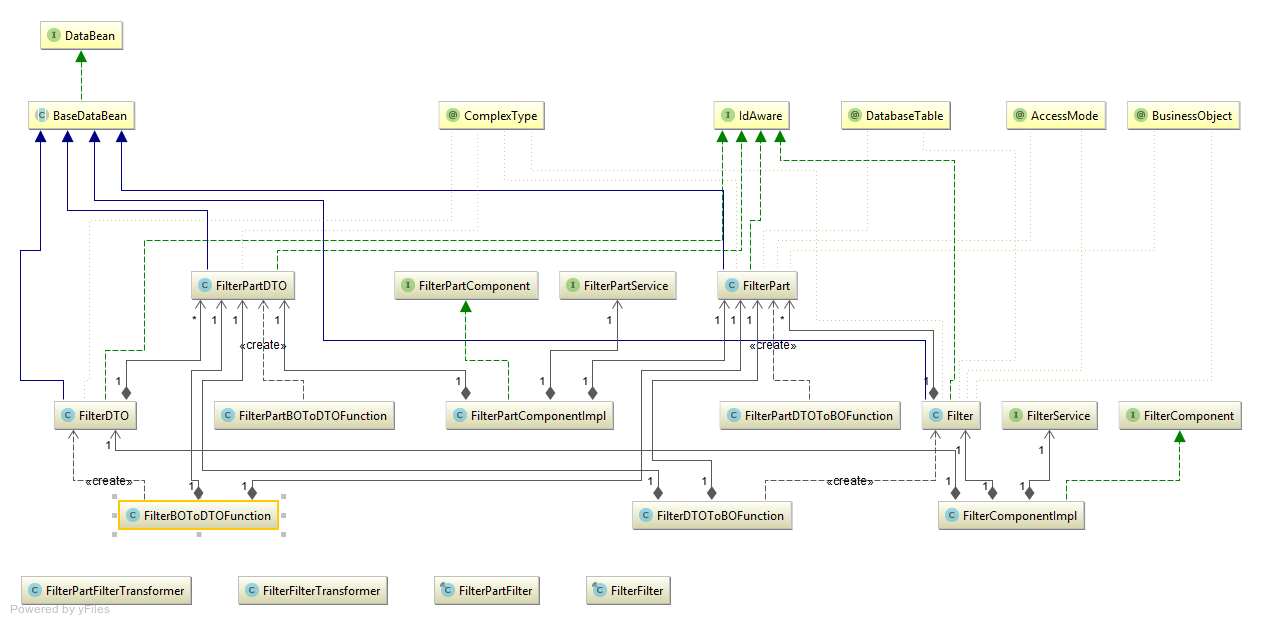
\includegraphics[width=\textheight]{diagrammrp.png}
\caption[]{Klassendiagramm}
\end{sidewaysfigure}

\subsection{Filter}
In dem MRP-Feature Masterdata wurde ein Feature hinzugefügt, welches zur Verwaltung von Filtern dient. Die Filter werden in der zentralen Datenbank von MRP gespeichert und über die Weboberfläche von MRP verwaltet, da die Filter zu den Masterdata-Features zählen. Die Filter dienen zur Filterung von MRP-Appointments. Jeder Filter beinhaltet die benötigten Filterkomponenten, welche für das Filtern der Daten verantwortlich sind. 
\subsection{Filterkomponenten}
Jeder Filter hat Filterkomponenten untergeordnet, welche die Informationen zu Filterart, Filtertyp und Filterwert enthalten. Diese Komponenten werden in einer Relation zu den Filtern in der Datenbank abgelegt. Die Filterkomponenten sind immer für einen bestimmten Filter zuständig und können nicht einzeln verwendet werden. Diese Filterkomponenten dienen zum Filtern von Appointments.
\subsection{Weboberfläche}
In der Weboberfläche von dem MRP-System werden die Filter und Filterkomponenten verwaltet. Die Oberfläche wird von G3 HIS bereitgestellt und bietet die Funktonalität von MRP. Mit Hilfe der Filter werden Appointments gesucht und angezeigt. Zukünftig sollen selektierte Appointments ins Microsoft Outlook exportiert werden können.



 
